\documentclass[10pt]{article}
\usepackage[hmargin=0.8cm,vmargin=0.2cm]{geometry}
\setlength{\parindent}{0pt}
\usepackage{listings,color}
\usepackage{graphicx}

\pagestyle{empty}

\begin{document}

\lstset{ %
language=Python,                % choose the language of the code
basicstyle=\footnotesize\ttfamily,       % the size of the fonts that are used for the code
stepnumber=1,                   % the step between two line-numbers. If it's 1 each line 
                                % will be numbered
numbersep=5pt,                  % how far the line-numbers are from the code
backgroundcolor=\color{white},  % choose the background color. You must add \usepackage{color}
showspaces=false,               % show spaces adding particular underscores
showstringspaces=false,         % underline spaces within strings
showtabs=false,                 % show tabs within strings adding particular underscores
frame=single,	                % adds a frame around the code
tabsize=2,	                % sets default tabsize to 2 spaces
captionpos=b,                   % sets the caption-position to bottom
breaklines=true,                % sets automatic line breaking
breakatwhitespace=false,        % sets if automatic breaks should only happen at whitespace
title=\lstname,                 % show the filename of files included with \lstinputlisting;
                                % also try caption instead of title
escapeinside={\%*}{*)},         % if you want to add a comment within your code
morekeywords={*,...}            % if you want to add more keywords to the set
}

\title{\bf Qjam: Python parallel framework for machine learning algorithms}
\author{Juan Batiz-Benet, Ali Yahya, Matt Sparks, Quinn Slack \\
{\tt \{jbenet,alive,msparks,sqs\}@cs.stanford.edu} \\
{\tt https://github.com/sqs/qjam}}

\maketitle

{\bf Goal.} Make it easy to prototype and run machine learning algorithms on clusters (in particular, the sparse autoencoder algorithm), without having to purchase an expensive software license for each node or use unpleasant programming languages. \\

{\bf Getting started.} Use {\tt corn} or any other machine with Python 2.6, Scipy, and Numpy.

\begin{verbatim}
$ ssh corn.stanford.edu
corn$ git clone http://github.com/sqs/qjam.git
corn$ cd qjam
corn$ python bin/sum-matrix-example.py 500 corn corn corn corn
Creating and permuting 500x500 matrix X with integers 1 .. 500^2
X = [[123370  86666  61991 ...,  13967  82760  99503]
     [  1748 210520 115701 ..., 161970  59732 216744]
  ...
Computed element sum of X = 31250125000
\end{verbatim}

{\bf Usage example: sparse autoencoder.} The sparse autoencoder algorithm is an unsupervised feature learning
algorithm. When applied to photographs, it learns features that
correspond to edge detectors.

\begin{verbatim}
corn$ python examples/sparse_autoencoder.py 10000 corn corn corn corn
   ...
At iterate  121    f=  9.74973D+00    |proj g|=  1.47347D-01
   ...
\end{verbatim}

%\begin{figure}[h]
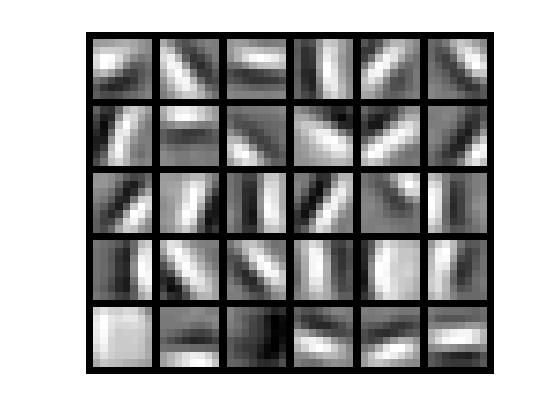
\includegraphics[scale=0.25]{sparseautoencoder_output.png}
%\end{figure}

{\bf Simple code example: distributed character count.} Run this with {\tt python char\_count.py}, after setting the env var $\quad$ {\tt PYTHONPATH=\$HOME/qjam}. It will distribute slices of a Shakespeare text to 4 {\tt corn} machines, wait for results from the workers, and then print the number of occurrences in the text of each character from {\tt a} to {\tt z}.

\begin{lstlisting}
import urllib2
from qjam import Master, DataSet
from qjam.master.remote_worker import RemoteWorker

def charcount(params, txtlines):
    cf = [0]*26
    for c in (''.join(txtlines)).lower():
        if c >= 'a' and c <= 'z':
            cf[ord(c)-ord('a')] += 1
    return cf
mapfunc = charcount

if __name__ == "__main__":
    ws = [RemoteWorker(h) for h in ['corn.stanford.edu']*4]
    url = 'http://stanford.edu/~sqs/qjam/shaks12.txt'
    txt = urllib2.urlopen(url).read().split("\n")
    cf = Master(ws).run(__import__('char_count'), None, DataSet(txt))
    for i,f in enumerate(cf):
        print "%s\t%d" % (chr(ord('a')+i), f)
\end{lstlisting}

\end{document}
